\section{Lissage d'une image}

\begin{enumerate}[questions, start=11]
\item On implémente le lissage par convolution sous Scilab dans le fichier \verb|functions.sci|:
  \begin{itemize}
  \item la fonction \verb|convolKernel(sigma, eta)| renvoie une matrice carrée $G$ dont les coefficients sont de la forme 
  \[ \dfrac{1}{2\pi\sigma^2}\exp{\left( -\dfrac{k^2 + l^2}{2\sigma^2} \right)} \]
  et vérifient tous $G_{i,j} \geq \eta$ ou sont nuls (où $\sigma =$ \verb|sigma| et $\eta = $ \verb|eta|);
  \item la fonction \verb|reflectMat(I, n)| renvoie une matrice au centre de laquelle on retrouve $I$. Les lignes et colonnes restantes sont remplies à partir de celles de $I$, par \og{}symétrie d'axe les bords de $I$\fg{};
  \item la fonction \verb|blur(I, sigma, eta)| calcule la convolée de $I$ par la gaussienne de paramètre $\sigma = $ \verb|sigma| tronquée à la précision $\eta = $ \verb|eta|.
  \end{itemize}
On peut voir quelques exemples sur des images ci-dessous:
\begin{figure}[!h]
\centering
  \begin{subfigure}{0.3\textwidth}
  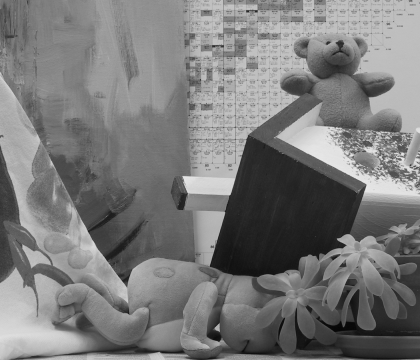
\includegraphics[width=\textwidth]{img/teddy-noblur.png}
  \caption{Image originale}
  \end{subfigure}\hfill
  \begin{subfigure}{0.3\textwidth}
  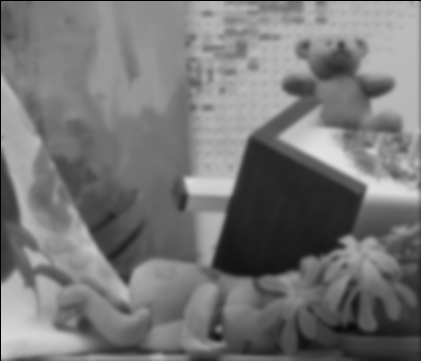
\includegraphics[width=\textwidth]{img/teddy-blur-2.png}
  \caption{Flou avec $\sigma = 2$}
  \end{subfigure}\hfill
  \begin{subfigure}{0.3\textwidth}
  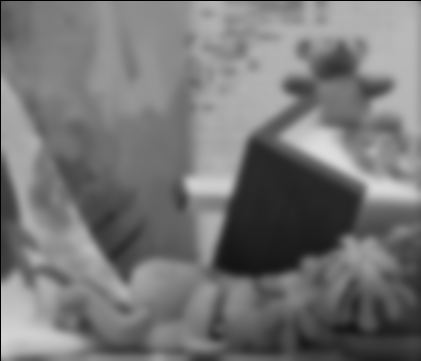
\includegraphics[width=\textwidth]{img/teddy-blur-4.png}
  \caption{Flou avec $\sigma = 4$}
  \end{subfigure}\\
  
  \begin{subfigure}{0.3\textwidth}
  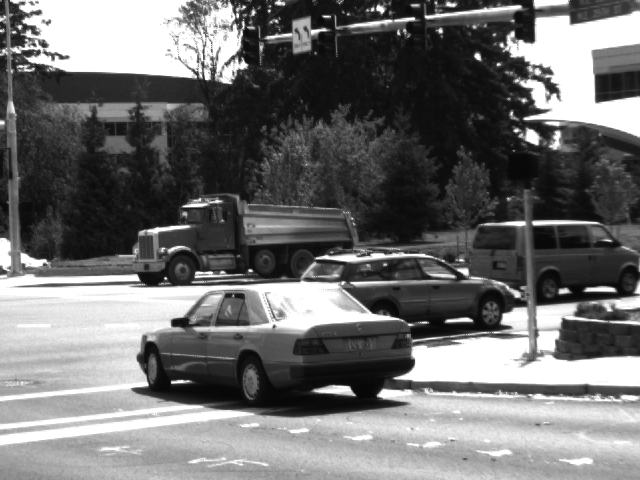
\includegraphics[width=\textwidth]{img/dumptruck-noblur.png}
  \caption{Image originale}
  \end{subfigure}\hfill
  \begin{subfigure}{0.3\textwidth}
  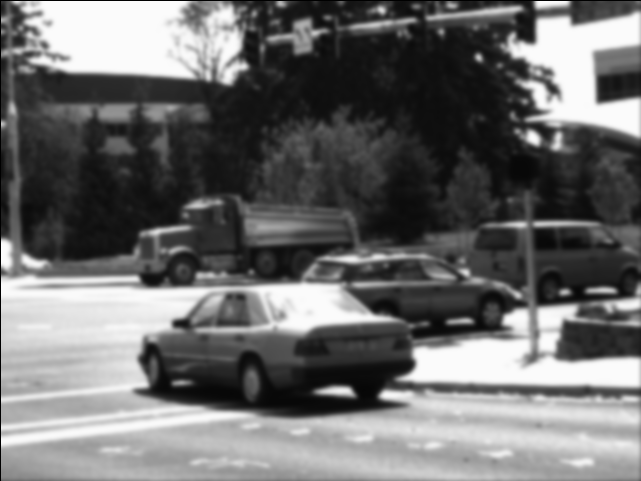
\includegraphics[width=\textwidth]{img/dumptruck-blur-2.png}
  \caption{Flou avec $\sigma = 2$}
  \end{subfigure}\hfill
  \begin{subfigure}{0.3\textwidth}
  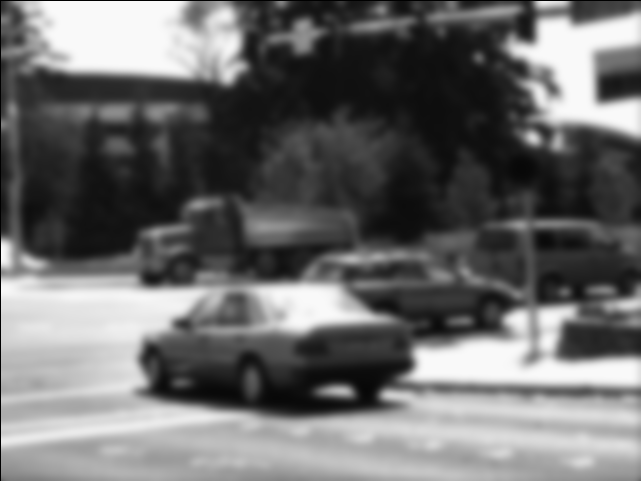
\includegraphics[width=\textwidth]{img/dumptruck-blur-4.png}
  \caption{Flou avec $\sigma = 4$}
  \end{subfigure}\\
  
  \begin{subfigure}{0.3\textwidth}
  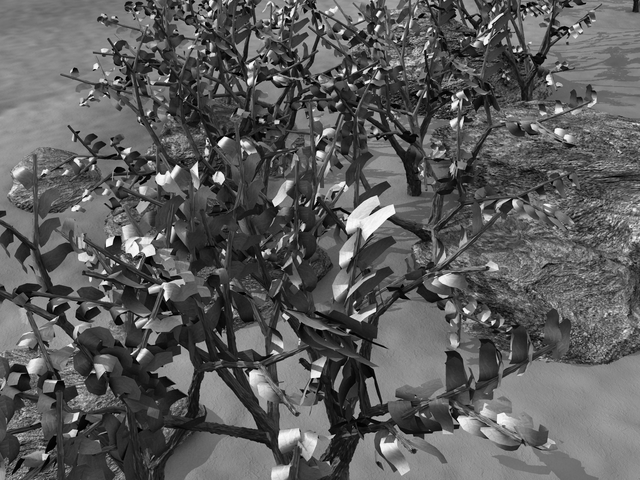
\includegraphics[width=\textwidth]{img/grove-noblur.png}
  \caption{Image originale}
  \end{subfigure}\hfill
  \begin{subfigure}{0.3\textwidth}
  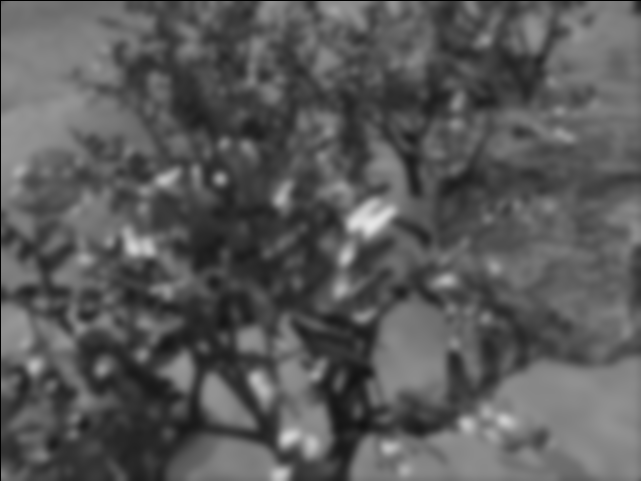
\includegraphics[width=\textwidth]{img/grove-blur-4.png}
  \caption{Flou avec $\sigma = 4$}
  \end{subfigure}\hfill
  \begin{subfigure}{0.3\textwidth}
  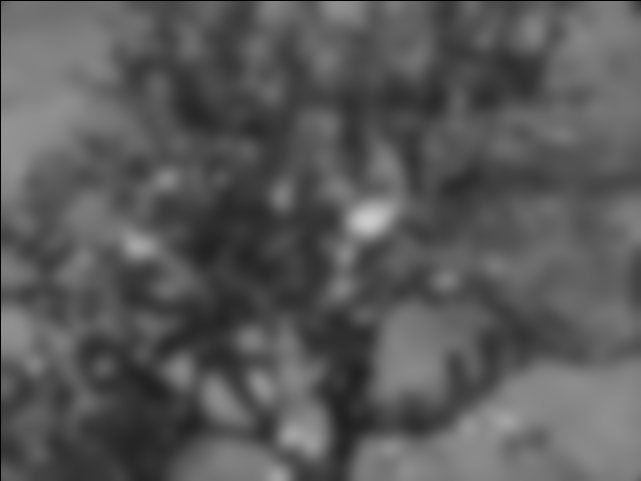
\includegraphics[width=\textwidth]{img/grove-blur-8.png}
  \caption{Flou avec $\sigma = 8$}
  \end{subfigure}
\end{figure}
\end{enumerate}

\begin{enumerate}[questions, start=13]
\item On travaille avec l'image suivante et sa version lissée. On applique l'algorithme de la question 7. 
\begin{figure}[!h]
\centering
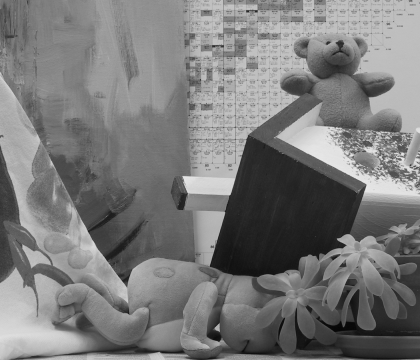
\includegraphics[width=.45\textwidth, height=6cm]{img/teddy-noblur} \hfill
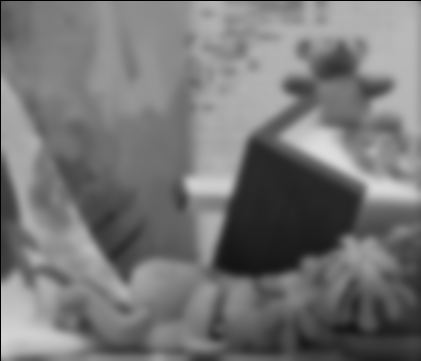
\includegraphics[width=.45\textwidth]{img/teddy-blur-4}\\
\bigskip
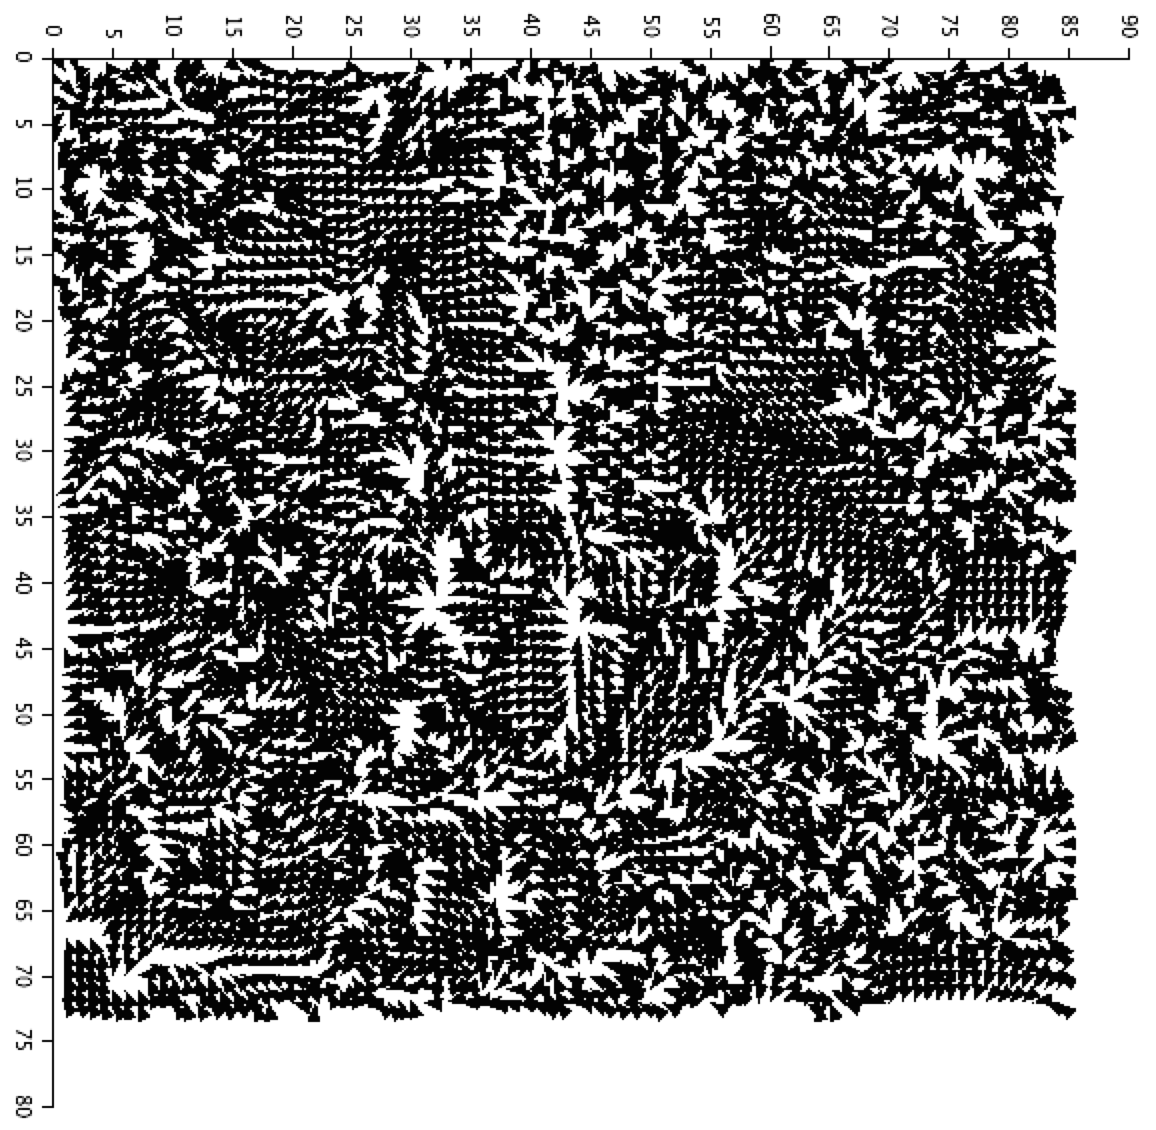
\includegraphics[width=.45\textwidth, height=6cm]{img/q13-result-1} \hfill
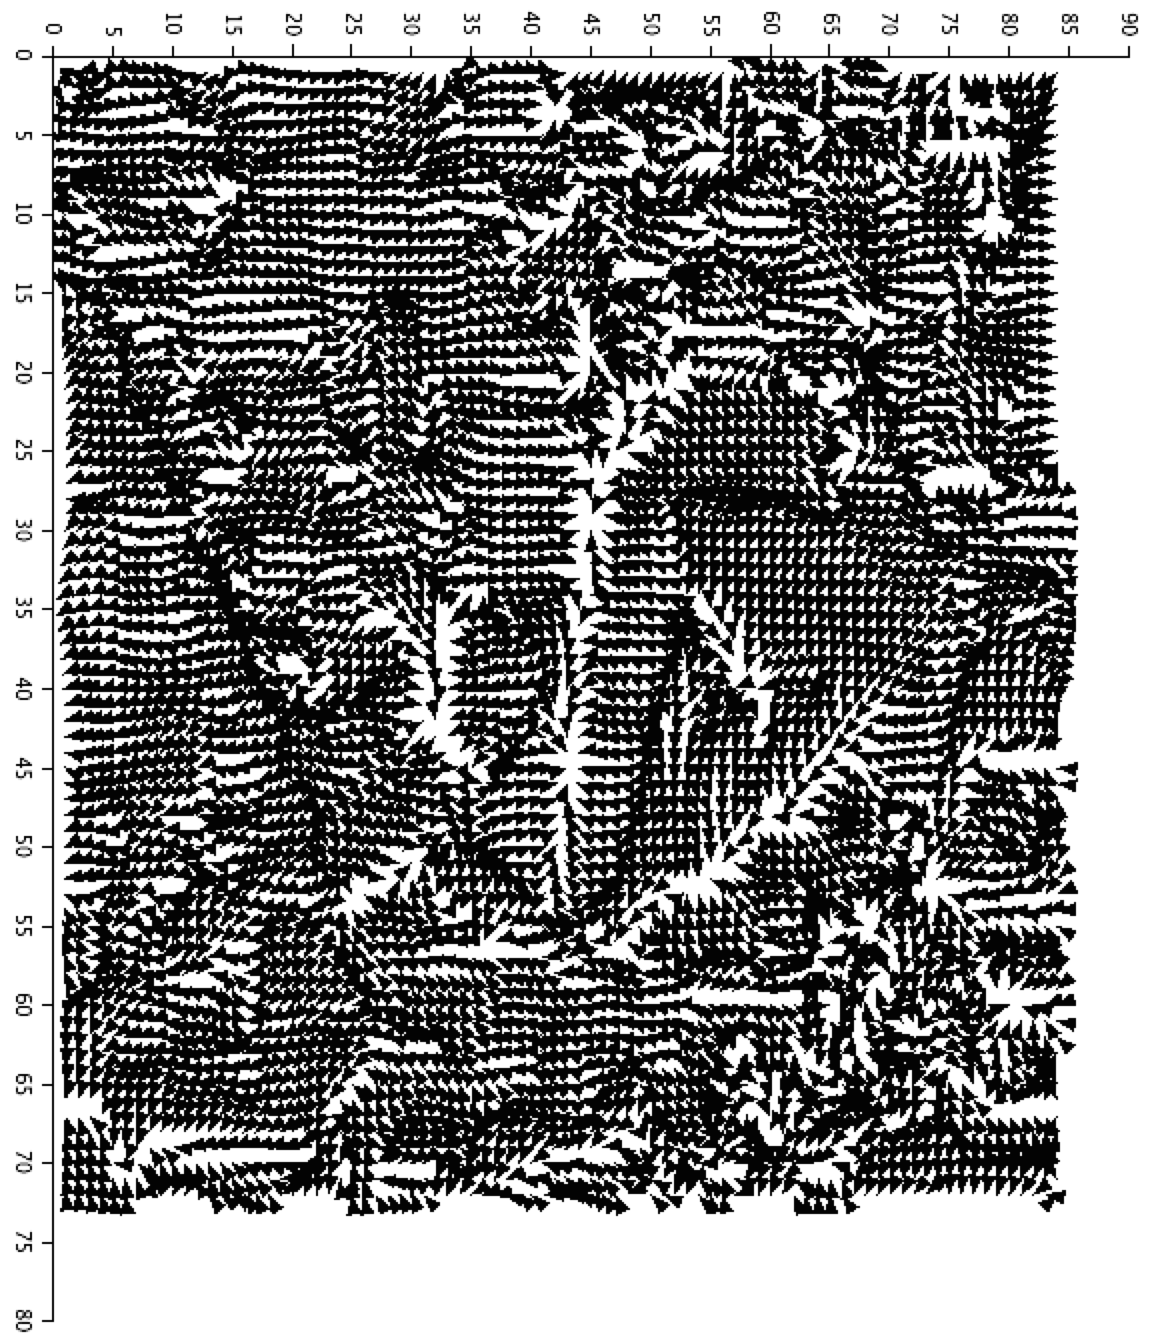
\includegraphics[width=.45\textwidth, height=6cm]{img/q13-result-2}
\end{figure}

On constate que le lissage permet d'avoir un flot optique mieux déterminé dans les régions moins contrastées. En revanche, on perd de l'information sur l'image au niveau des zones des contrastées. Par exemple, le mouvement de la cheminée que l'on peut observer sur le résultat de gauche n'est plus visible sur celui de droite.

\item On implémente l'algorithme, dans le fichier \verb|functions.sci|, en plusieurs fonctions qui seront appelées par une fonction globale:
  \begin{itemize}
  \item \verb|simpleSmall(I,f)| réduit la taille d'une matrice d'un facteur \verb|f|;
  \item \verb|simpleBig(I,f)| agrandit la taille d'une matrice d'un facteur \verb|f|;
  \item \verb|applyNegativeFlow(I,u,v)| retranche le flot $(u,v)$ à la matrice $I$;
  \item \verb|smartFlow(I1, I2)| calcule le flot optique entre les deux images de la façon décrite dans l'énoncé.
  \end{itemize}
On a testé ce programme sur la même image que précédemment. Le résultat est visible sur la figure \vref{fig:q14-results}.
\begin{figure}
\centering
  \begin{subfigure}{.6\textwidth}
  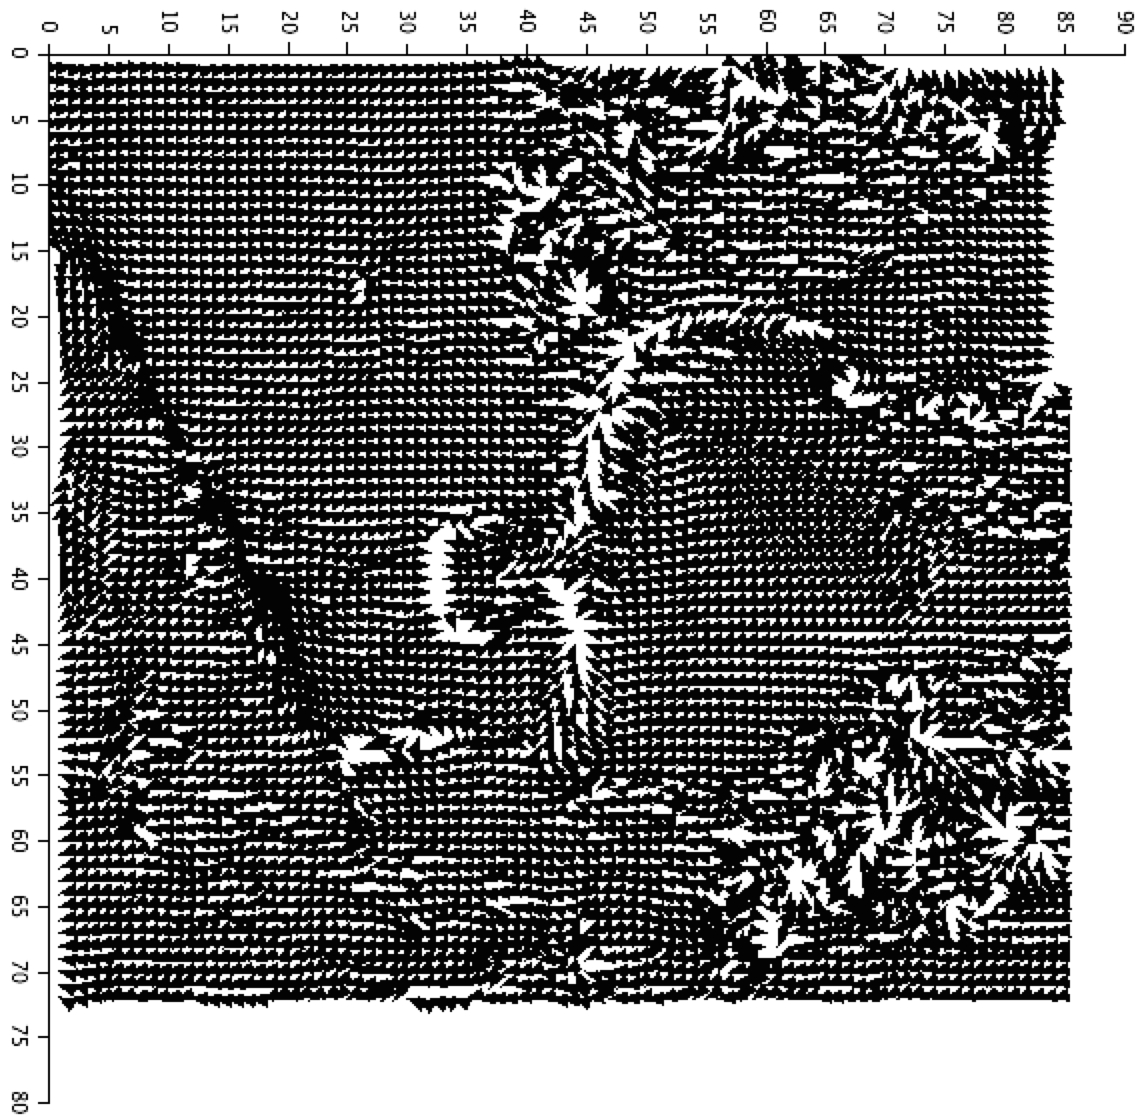
\includegraphics[width=\textwidth]{img/q14-results}
  \caption{Résultat global.}
  \end{subfigure} \\
  \begin{subfigure}{.6\textwidth}
  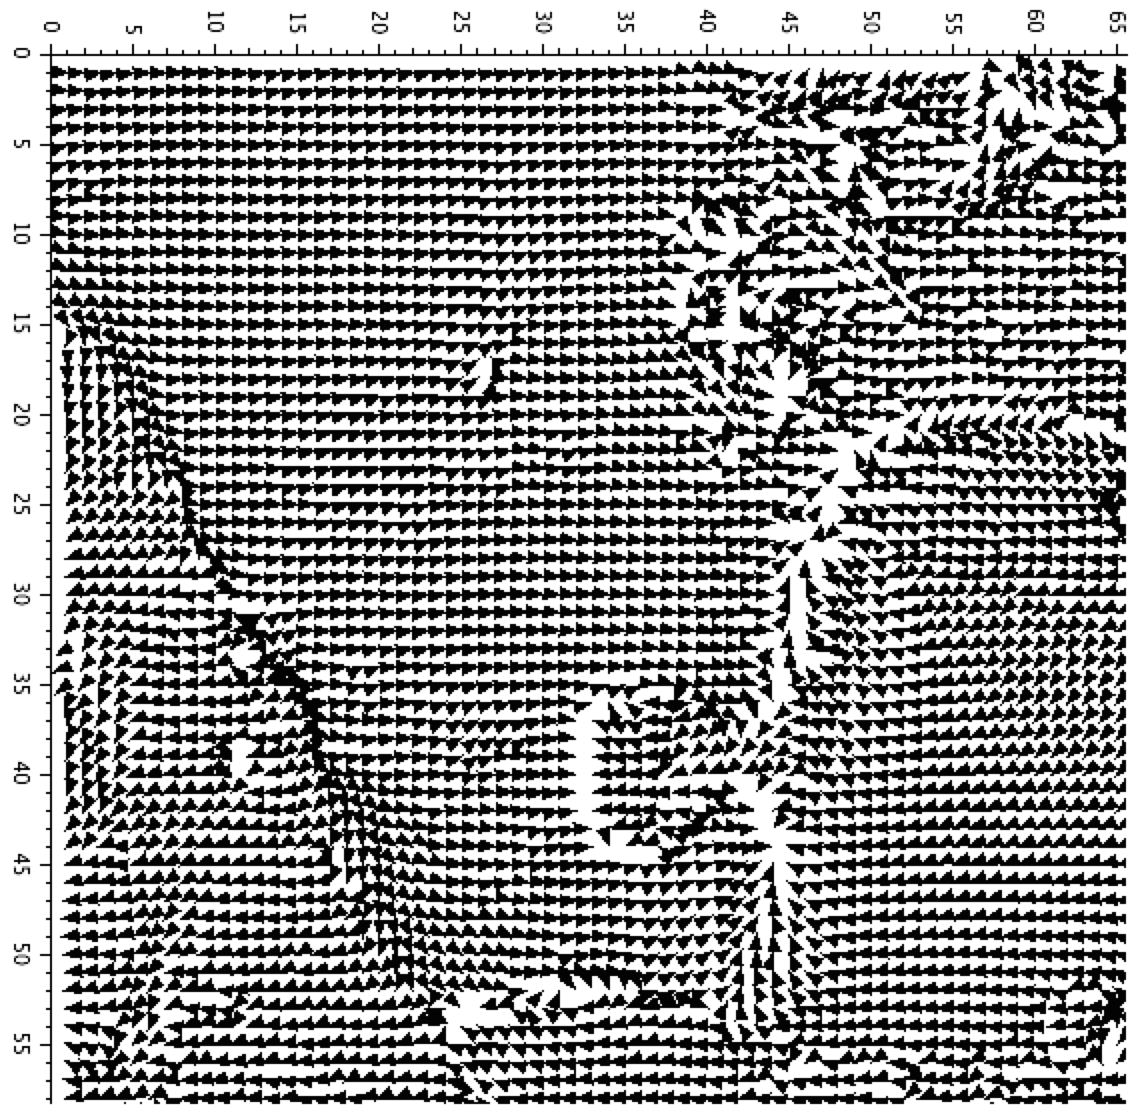
\includegraphics[width=\textwidth]{img/q14-results-zoom}
  \caption{Zoom sur une partie de la matrice.}
  \end{subfigure}
\caption{Résultats de la question 14.\label{fig:q14-results}}
\end{figure}
On remarque que le flot est plus régulier que dans les questions 7 ou 13, et la partie agrandie nous montre que les zones où l'intensité est quasi-constante sont bien traitées dans le sens où le flot est constant et non \og{}chaotique\fg{} comparé aux résultats des questions précédentes.
\end{enumerate}